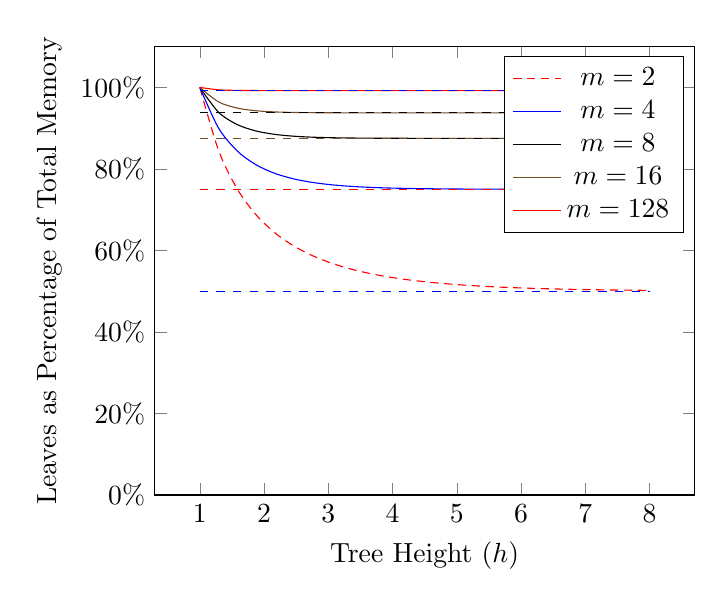
\begin{tikzpicture}
	\begin{axis}
		[
			xlabel={Tree Height ($h$)},
			ylabel={Leaves as Percentage of Total Memory},
			xtick distance=1,
			yticklabel={%
				\pgfmathparse{\tick*100}%
				\pgfmathprintnumber{\pgfmathresult}%
				\%%
			},
			domain=1:8,
			ymin=0,
			smooth
		]
		\pgfplotsinvokeforeach{2,4,8,16,128} {
			\addplot+[cycle list name=color list, mark=none]
				{#1^(x-1) / ((1-#1^x)/(1-#1))};
			\addlegendentry{$m=#1$}
		}
		\pgfplotsset{cycle list shift=-5}
		\pgfplotsinvokeforeach{2,4,8,16,128} {
			\addplot+[cycle list name=color list, mark=none, dashed]
				{1-(1/#1)};
		}
	\end{axis}
\end{tikzpicture}
